

\chapter{Results}
In this chapter we present the results from our experiments on different types of imbalanced datasets. We first start by showing the results on the balanced model so as to set the baseline of comparisons. A discussion then follows on the under-sampled and over-sampled cases, ending with the transfer learning results for perturbations with different models. The chapter is then concluded with the results for the cases where classes have similar features, and, therefore, share overlapping distributions.


\section{Baseline model}

Canonical models assume that every object in the dataset are sampled from similar distributions. However, in real-life situations, even though the number of samples is the same for each label, they could still be poorly represented by the lack of a clear structure. This often leads to differences in the output for each specific class \cite{krawczyk2016learning}. On this way, a superficially balanced dataset does not guarantee that the model will equally generalise across all classes.We use the results of the balanced network on adversarial attacks as the baseline
to evaluate whether imbalanced CNNs are more or less vulnerable to adversarial
learning
\begin{figure}[H]
	\centering
	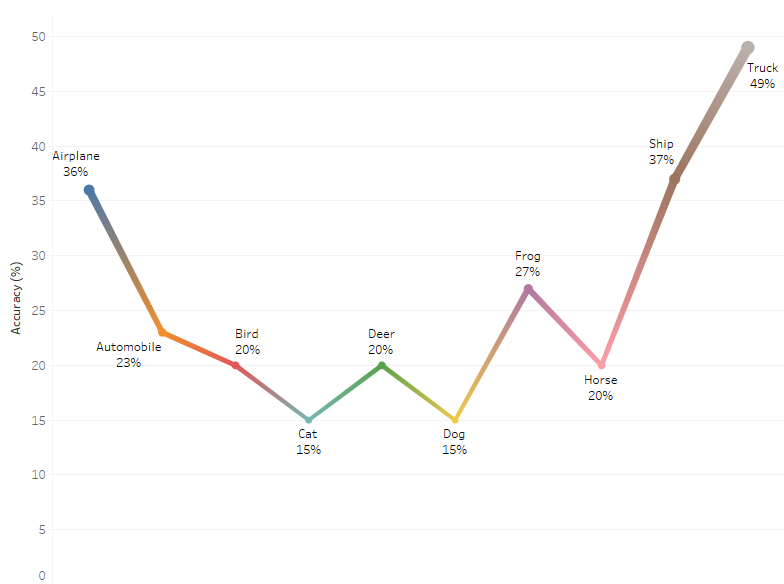
\includegraphics[scale=0.7]{balanced_perturbed.png}
	\caption{Individual class perturbed accuracy on the balanced model}
	\label{fig:balanced_perturbed}
\end{figure}

Figure ~\ref{fig:balanced_perturbed} shows that the accuracy for all classes is drastically reduced when the balanced model is presented with adversarial examples. Even though there is equally distributed number of samples for each class, the adversarial attack forces the domain shift of each individual sample towards different regions in space, causing a misclassification of the current label.

\section{Under-sampling and over-sampling models}


The results on both under-sampled and over-sampled network has show some interesting properties of adversarial attacks. 
Table ~\ref{tbl:results} shows that models with under-sampled datasets were even more vulnerable than balanced networks. Figure ~\ref{fig:relative_difference} shows the relative difference for all the three different networks (balanced, under-sampled and over-sampled). Values were calculated by finding the difference between the perturbed accuracy and the non-perturbed accuracy of each class model. They represent the percentage on which the initial accuracy was reduced. The under-sampled model had the higher relative difference on average, which shows that the imbalanced nature of the dataset ended-up increasing the vulnerability to adversarial attacks

Perturbation on the over-sampling case, on the other hand, had a weaker effect, as the small push caused by our $\epsilon$ was not enough to move points to outside of their distributions. Objects of the over-sampled classes would need bigger steps in order to successfully create an adversary that leads to a wrong classification label. Accuracy for
most of the over-sampling cases was around 45\% and the relative difference was the lowest of all three models, which shows robustness of the target over-sampled class.

Class imbalanced models are naturally affected by the false positive and false negative trade off shown on figure \ref{fig:class_dist}. The decision boundaries on such models favour the class with more samples and, hence, increases the accuracy for one class while decreasing for the other class. The area under the curve for misclassified examples on the under-sampled distribution is bigger, and it is caused by the suboptimal exploration of feature space of that class. This effect is exploited by adversaries as there is an increase on the misclassification rate of distributions with lower amplitude. An under-sample of a specific label causes its distribution to be squished into space and, hence, have less impact on the definition of decision boundaries.

\begin{figure}[H]
	\centering
	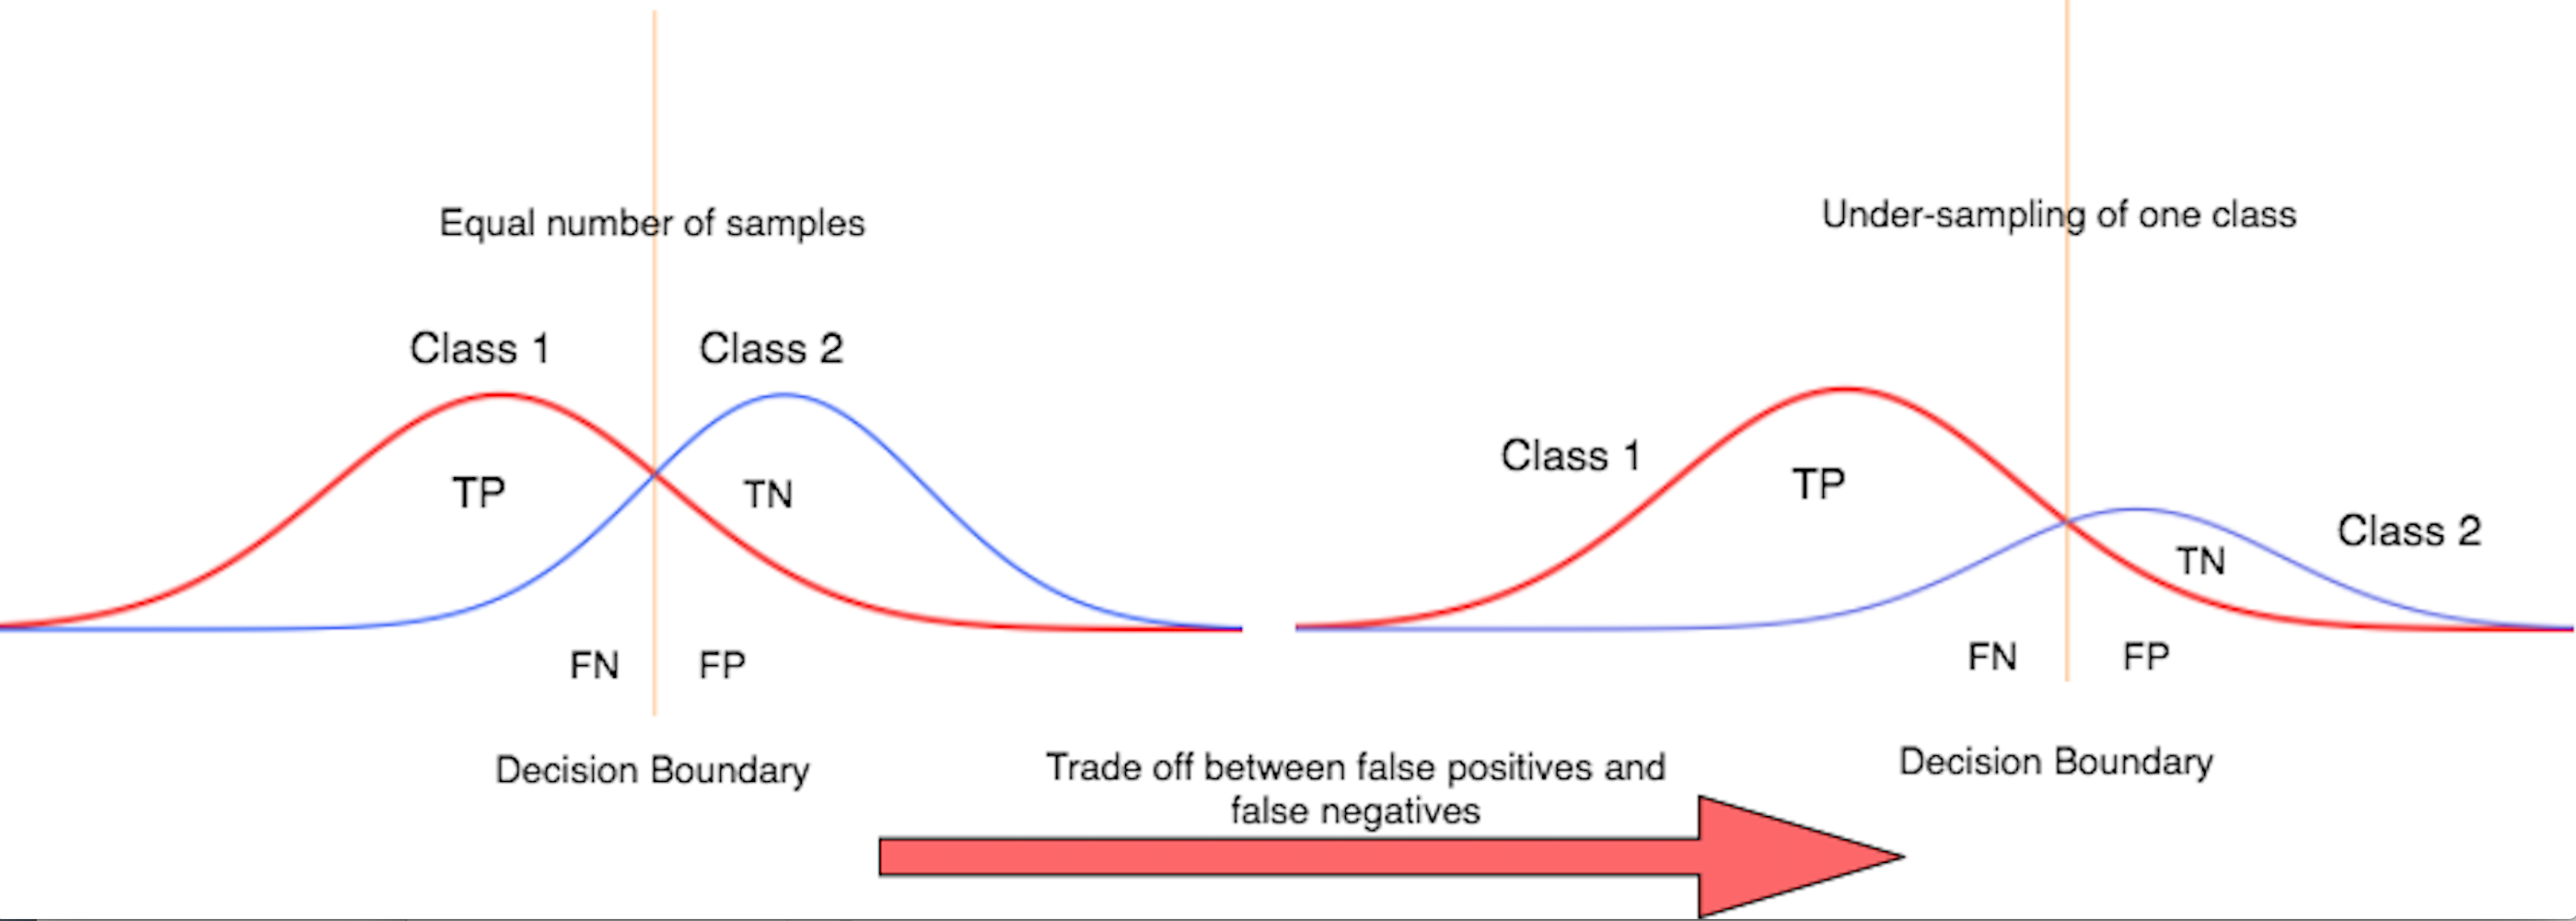
\includegraphics[scale=0.32]{class_dist.png}
	\caption{Dataset imbalance causes models to perform adjustments of decision boundaries leading to an increase on accuracy of the majority class and decrease on the minority class.}
	\label{fig:class_dist}
\end{figure}



\begin{table}[H]
	\centering
	
	\begin{tabular}{lccccc}
		\toprule
		&\multicolumn{2}{c}{Different Model}
		&\multicolumn{3}{c}{Same Model}
		\\\cmidrule(r){2-3}\cmidrule(l){4-6}
		Class Label &Undersample &Oversample &Balanced &Undersample &Oversample \\
		\midrule
		0 - Airplane &60\%& 87\% &36\%& 19\%    & 61\% \\
		1 - Automobile &64\%& 91\% &23\%& 16\%    & 63\% \\
		2 - Bird &38\%& 73\% &20\%& 9.4\%    & 27\% \\
		3 - Cat &21\%& 72\% &11\%& 0.5\%    & 19\% \\
		4 - Deer &58\%& 80\% &20\%& 9.8\%    & 20\% \\
		5 - Dog &47\%& 76\% &15\%& 9\%    & 38\% \\
		6 - Frog &76\%& 88\% &27\%& 20\%    & 49\% \\
		7 - Horse &59\%& 88\% &20\%& 18\%    & 52\% \\
		8 - Ship &69\%& 89\% &37\%& 19\%    & 59\% \\
		9 - Truck &46\%& 87\% &49\%& 21\%    & 54\% \\
		\bottomrule
	\end{tabular}
	\caption{Results for the two different sources of perturbations along with the two different imbalanced datasets}
	\label{tbl:results}
\end{table}


The increased number of samples of the over-sampled label, causes the network to perform a trade-off when optimizing its loss function. For instance, the decision boundary is chosen in order to minimize the total error of the network. The cost function is lower when the decision boundary minimizes the misclassification of the majority class, as there is a higher number of samples. This phenomenon is well explained by figure ~\ref{fig:class_dist}, and it could be one of the factors explaining the higher resilience of over-sampled networks.

\begin{figure}[H]
	\centering
	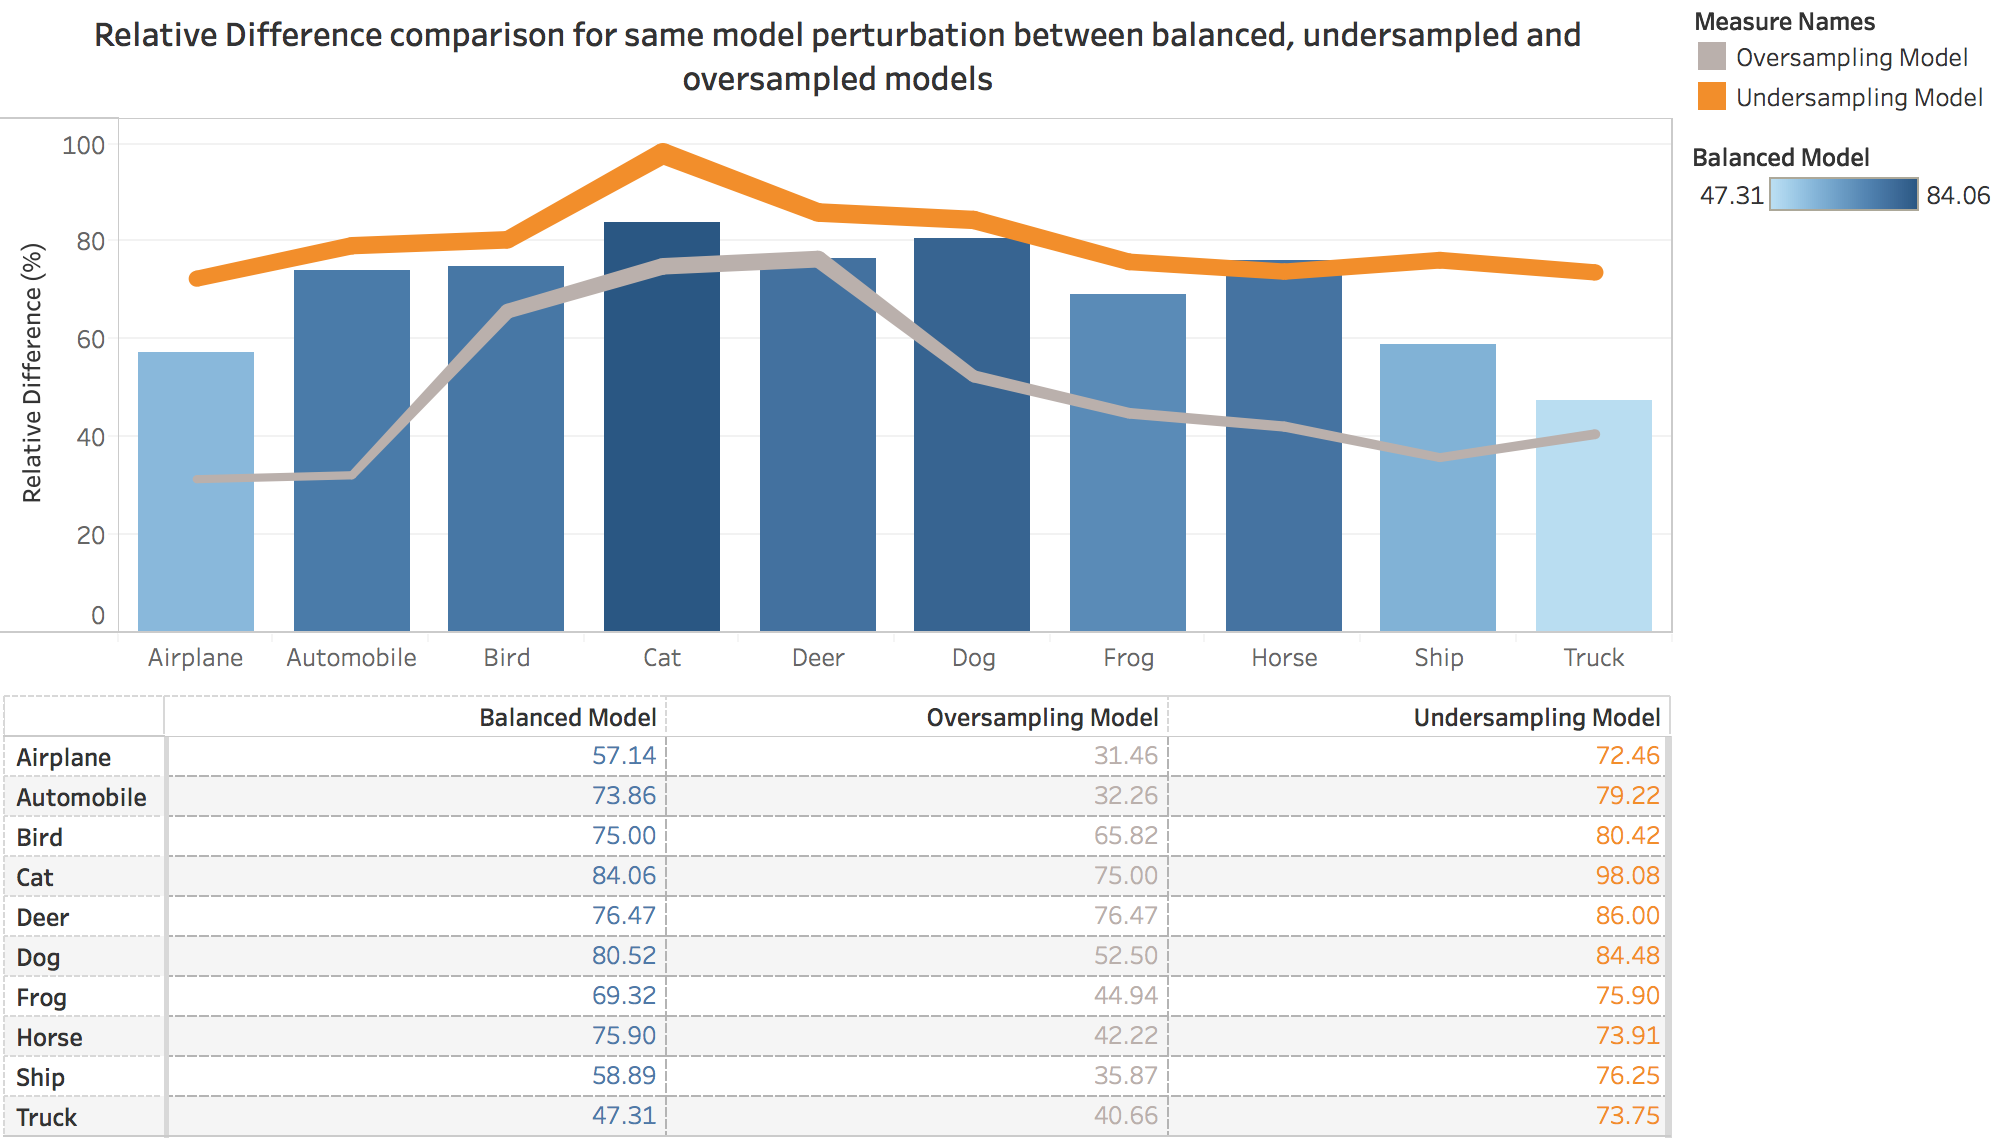
\includegraphics[scale=0.3]{rel_diff_graph.png}
	\caption{Relative difference for each model. Higher numbers means more vulnerability}
	\label{fig:relative_difference}
\end{figure}

\section{Transfer learning}

Chapter 4 discussed different ways in which one algorithm could learn from existing models. Black-box attack is when the attacker has no knowledge of the underlying model that he/she wants to attack and the best way to learn the gradient information is by querying the target and training a new model with its outputs. White-box attack is when the same model is used to extract the gradient for the gradient sign method.

The use of a different model (black-box) for creating adversaries has shown less effective when compared to the same model (white-box) attack. As the overall gradient have not only different direction but also magnitudes, the attacked system has proven to be more robust. The experiment reveals that although gradient sign method is quite effective for fooling networks it does require a good amount of knowledge from the underlying training parameters so as to unleash its full potential.

Attacking an under-sampled network with the gradient of the balanced network did not show to be as effective as using the same model's gradient. The average accuracy of an under-sampled model attack with adversaries generated from a different network was 53.8\% while the same metric was 25.8\% for the same model attack. Even that our training samples are within the same data domain, there are still huge differences on the gradients learned from the network. 

\section{Overlapping distributions}
The results for the balanced network on figure~\ref{fig:conf_matrix_full} shows that for the pairs cat/dog and automobile/truck there is already a natural misclassification between one another. For instance 13\% of dog samples were misclassified as cat in the original balanced model. Our experiment demonstrates that the adversarial attacks intensify this phenomena in only one of the classes of the pair. While for both under-sampled cat and truck the number of samples misclassified with the similar class has increased, the same did not happen with dog and automobile. Figure~\ref{fig:overlap} shows that cats are increasingly misclassified as dogs when under-sampling on the cat class is used. While on the cat under-sampling case the percentage of samples misclassified as dogs increased from 31\% to 39\%, the same number decreased from 38\% to 32\% on the dog under-sampling test.
\begin{figure}
	\centering
	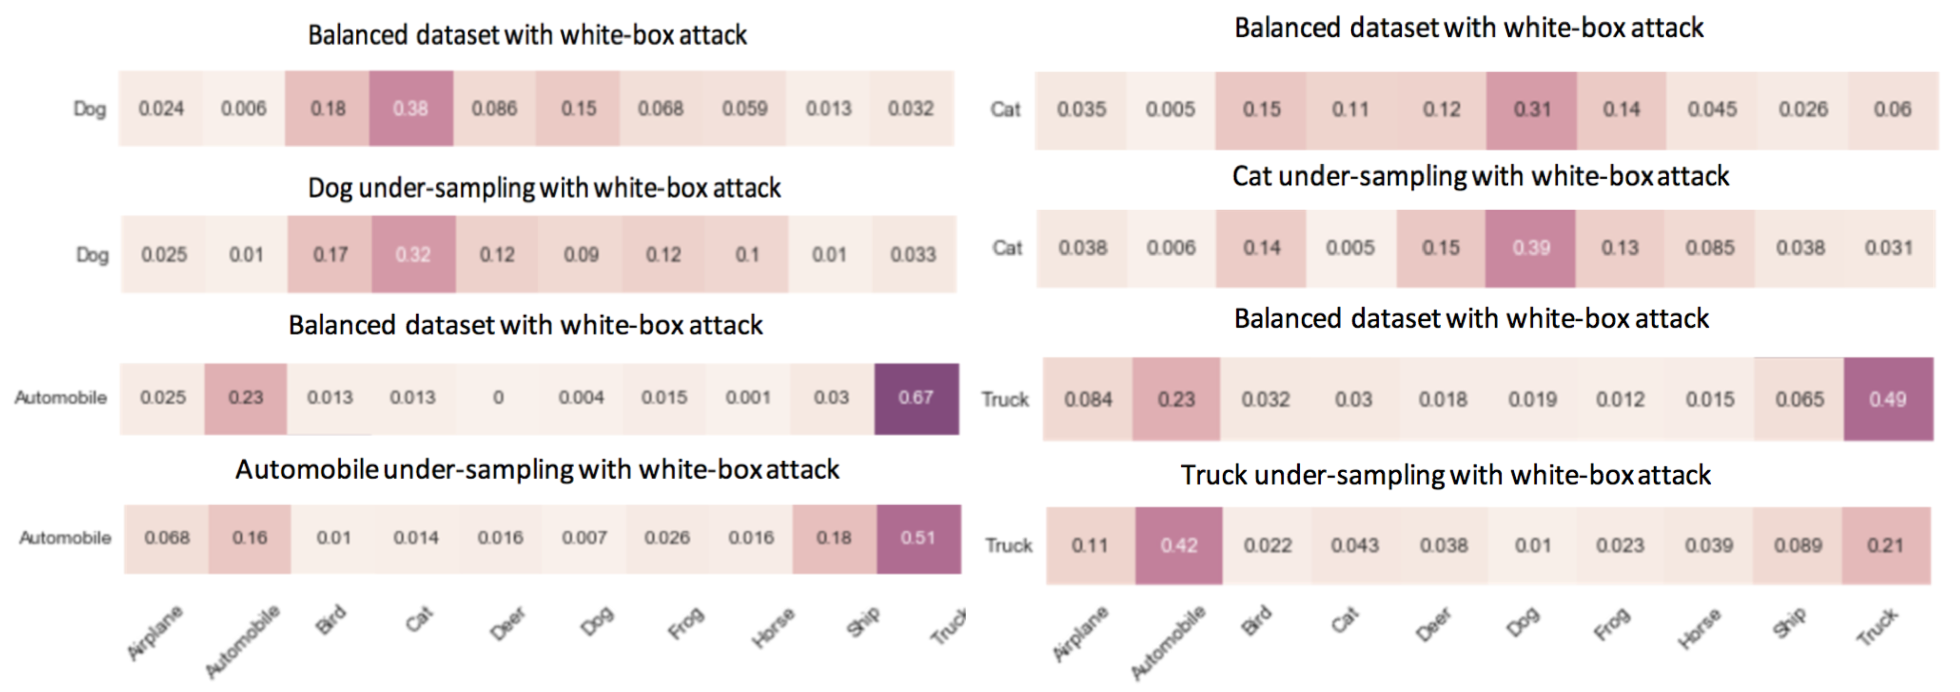
\includegraphics[height=4.5cm]{overlapping_all.png}
	\caption{Under-sample on cat and truck increases misclassification to similar classes, while dog and automobile does not.}
	\label{fig:overlap}
\end{figure}